%!TEX root = ../Report.tex
\chapter{Demo of the Cloud Storage Mounts}
\label{demos}
In this chapter, I will demonstrate mounting directories from various cloud storage providers using the tool RClone. Since I was unsuccessful in implementing OCamlFUSE, demonstrations using OCamlFUSE will not be included in this chapter.
\section{Google Drive}
The Google Drive implementation is what I started with in lab reports. Please refer to \ref{rclonegdrivedemo} for the Google Drive demo using RClone.
\section{Dropbox}
Next, I move on to Dropbox to demonstrate that RClone has implemented mounting for directories and files stored in the Dropbox cloud storage provider. The following is the terminal output.\\
\begin{verbatim}
$ rclone config
Current remotes:

Name                 Type
====                 ====
remote               drive

e) Edit existing remote
n) New remote
d) Delete remote
r) Rename remote
c) Copy remote
s) Set configuration password
q) Quit config
e/n/d/r/c/s/q> n
name> dpremote
Type of storage to configure.
Enter a string value. Press Enter for the default ("").
Choose a number from below, or type in your own value
1 / A stackable unification remote, which can appear to merge the 
contents of several remotes
   \ "union"
2 / Alias for an existing remote
   \ "alias"
3 / Amazon Drive
   \ "amazon cloud drive"
4 / Amazon S3 Compliant Storage Provider (AWS, Alibaba, Ceph, 
Digital Ocean, Dreamhost, IBM COS, Minio, etc)
   \ "s3"
5 / Backblaze B2
   \ "b2"
6 / Box
   \ "box"
7 / Cache a remote
   \ "cache"
8 / Dropbox
   \ "dropbox"
9 / Encrypt/Decrypt a remote
   \ "crypt"
10 / FTP Connection
   \ "ftp"
11 / Google Cloud Storage (this is not Google Drive)
   \ "google cloud storage"
12 / Google Drive
   \ "drive"
13 / Hubic
   \ "hubic"
14 / JottaCloud
   \ "jottacloud"
15 / Koofr
   \ "koofr"
16 / Local Disk
   \ "local"
17 / Mega
   \ "mega"
18 / Microsoft Azure Blob Storage
   \ "azureblob"
19 / Microsoft OneDrive
   \ "onedrive"
20 / OpenDrive
   \ "opendrive"
21 / Openstack Swift (Rackspace Cloud Files, Memset Memstore, OVH)
   \ "swift"
22 / Pcloud
   \ "pcloud"
23 / QingCloud Object Storage
   \ "qingstor"
24 / SSH/SFTP Connection
   \ "sftp"
25 / Webdav
   \ "webdav"
26 / Yandex Disk
   \ "yandex"
27 / http Connection
   \ "http"
Storage> dropbox
** See help for dropbox backend at: https://rclone.org/dropbox/ **

Dropbox App Client Id
Leave blank normally.
Enter a string value. Press Enter for the default ("").
client_id>
Dropbox App Client Secret
Leave blank normally.
Enter a string value. Press Enter for the default ("").
client_secret>
Edit advanced config? (y/n)
y) Yes
n) No
y/n> y
Upload chunk size. (< 150M).

Any files larger than this will be uploaded in chunks of this size.

Note that chunks are buffered in memory (one at a time) so rclone can
deal with retries.  Setting this larger will increase the speed
slightly (at most 10% for 128MB in tests) at the cost of using more
memory.  It can be set smaller if you are tight on memory.
Enter a size with suffix k,M,G,T. Press Enter for the default ("48M").
chunk_size>
Impersonate this user when using a business account.
Enter a string value. Press Enter for the default ("").
impersonate>
Remote config
Use auto config?
* Say Y if not sure
* Say N if you are working on a remote or headless machine
y) Yes
n) No
y/n> y
If your browser doesn't open automatically go to the following link: 
http://127.0.0.1:53682/auth
Log in and authorize rclone for access
Waiting for code...
Got code
--------------------
[dpremote]
type = dropbox
token = {"access_token":"yeGRic_xxxx-M-xxxx-T","token_type":"bearer",
"expiry":"0001-01-01T00:00:00Z"}
--------------------
y) Yes this is OK
e) Edit this remote
d) Delete this remote
y/e/d> y
\end{verbatim}
Refer to Figure \ref{fig:dropbox1}, Figure \ref{fig:dropbox2}, and Figure \ref{fig:dropbox3} for visualization of what occurs when the browser appears when user runs the commands above.
\begin{figure}[htb]
  \centering
  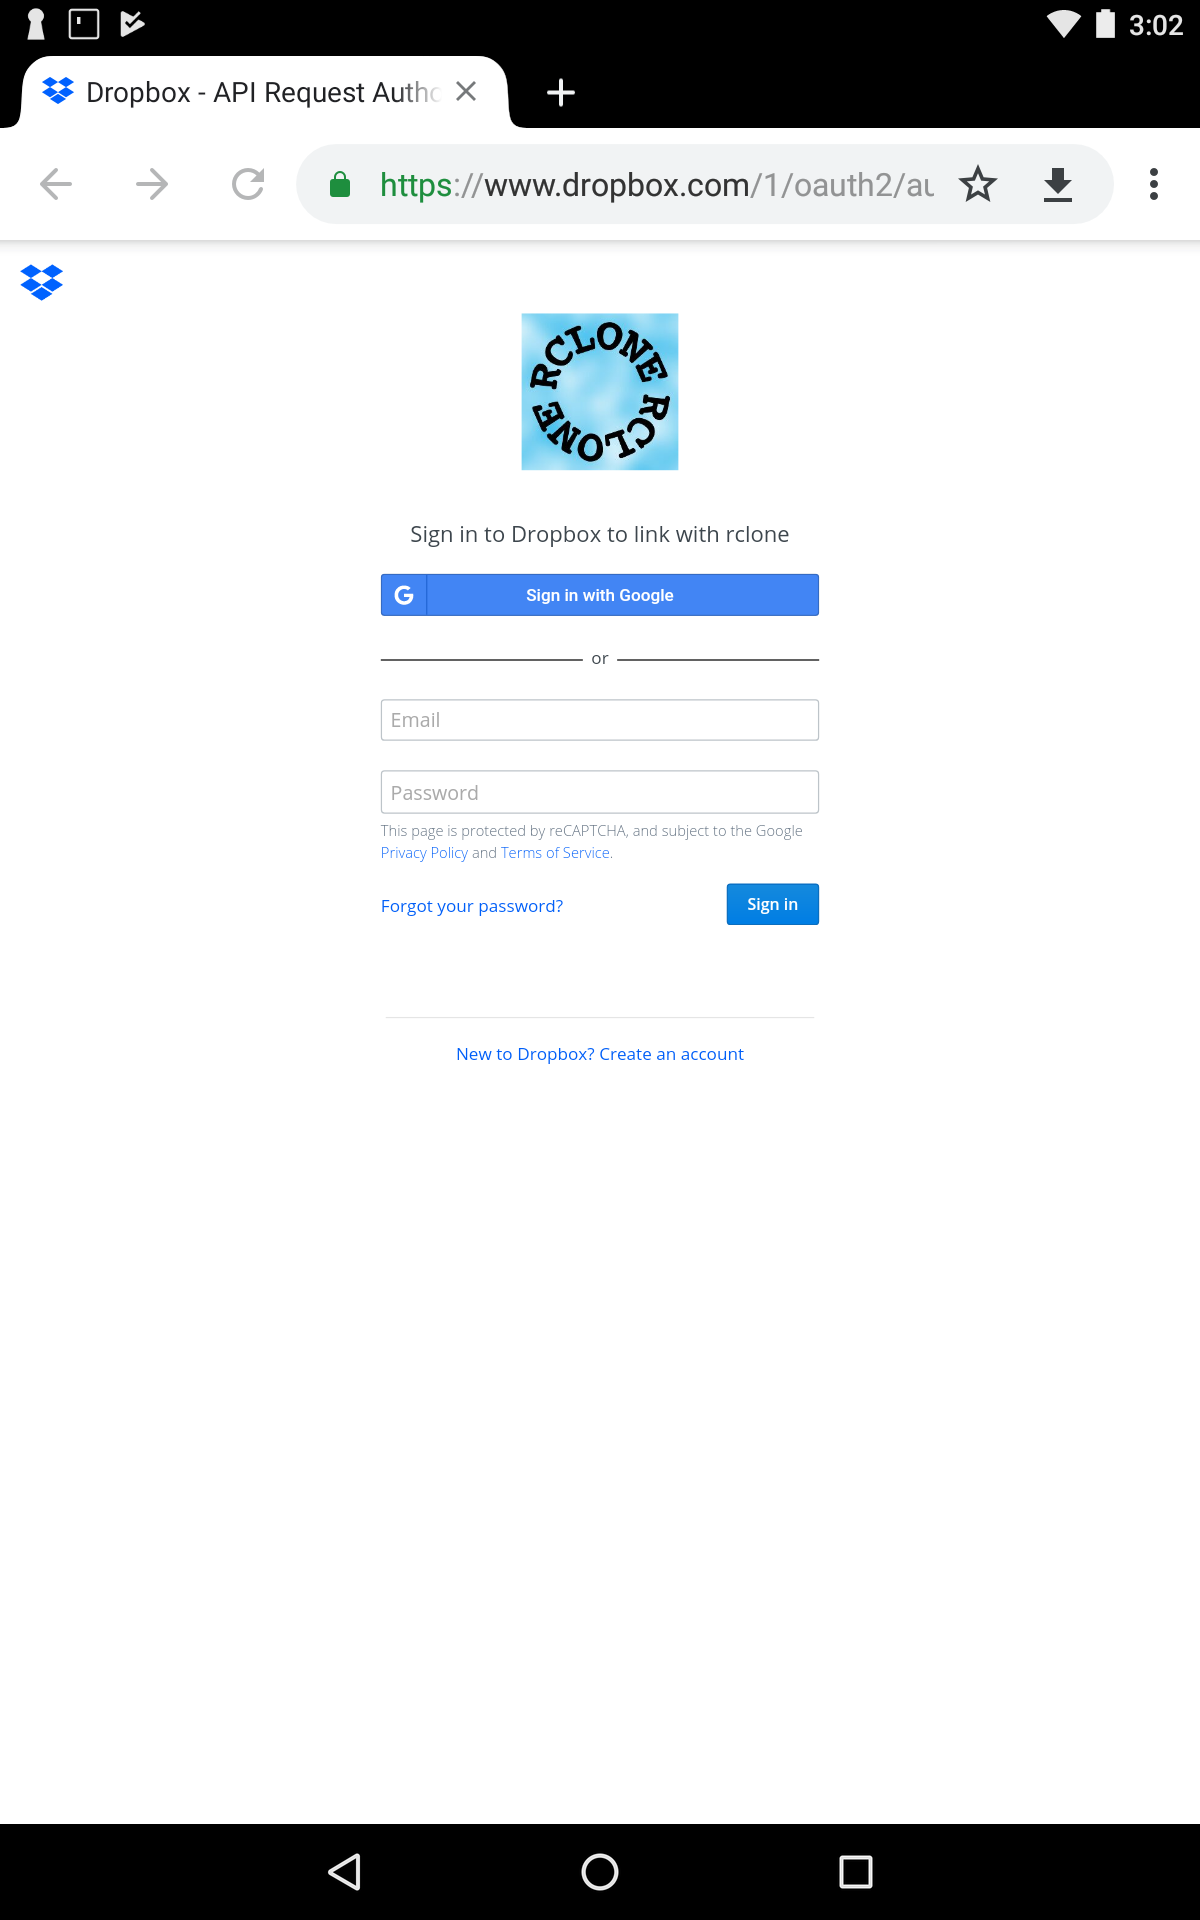
\includegraphics[scale=0.2]{images/dropbox1.png}
  \caption{Browser appears prompting for Dropbox credentials}
  \label{fig:dropbox1}
\end{figure}
\begin{figure}[htb]
  \centering
  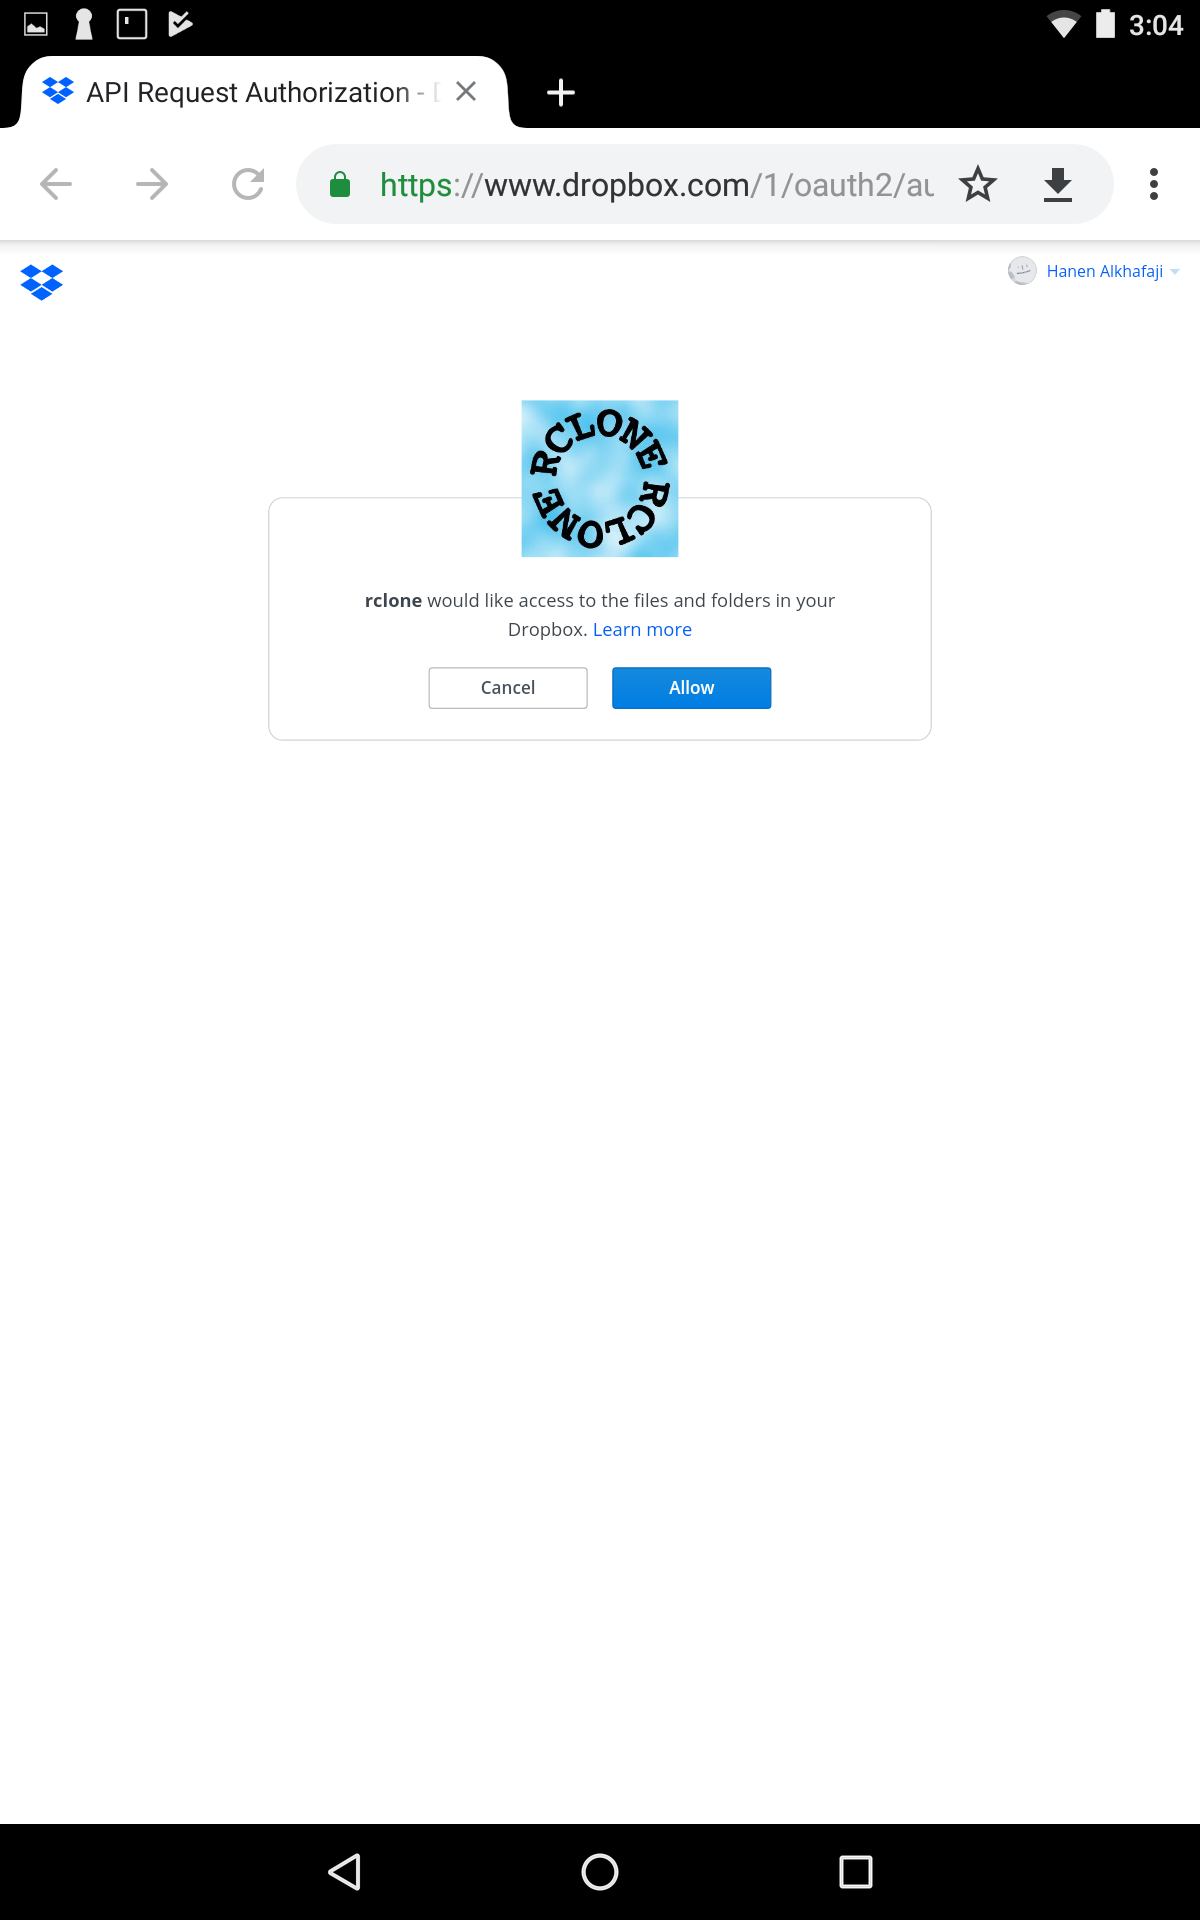
\includegraphics[scale=0.2]{images/dropbox2.png}
  \caption{RClone requests permission to access Dropbox content}
  \label{fig:dropbox2}
\end{figure}
\begin{figure}[htb]
  \centering
  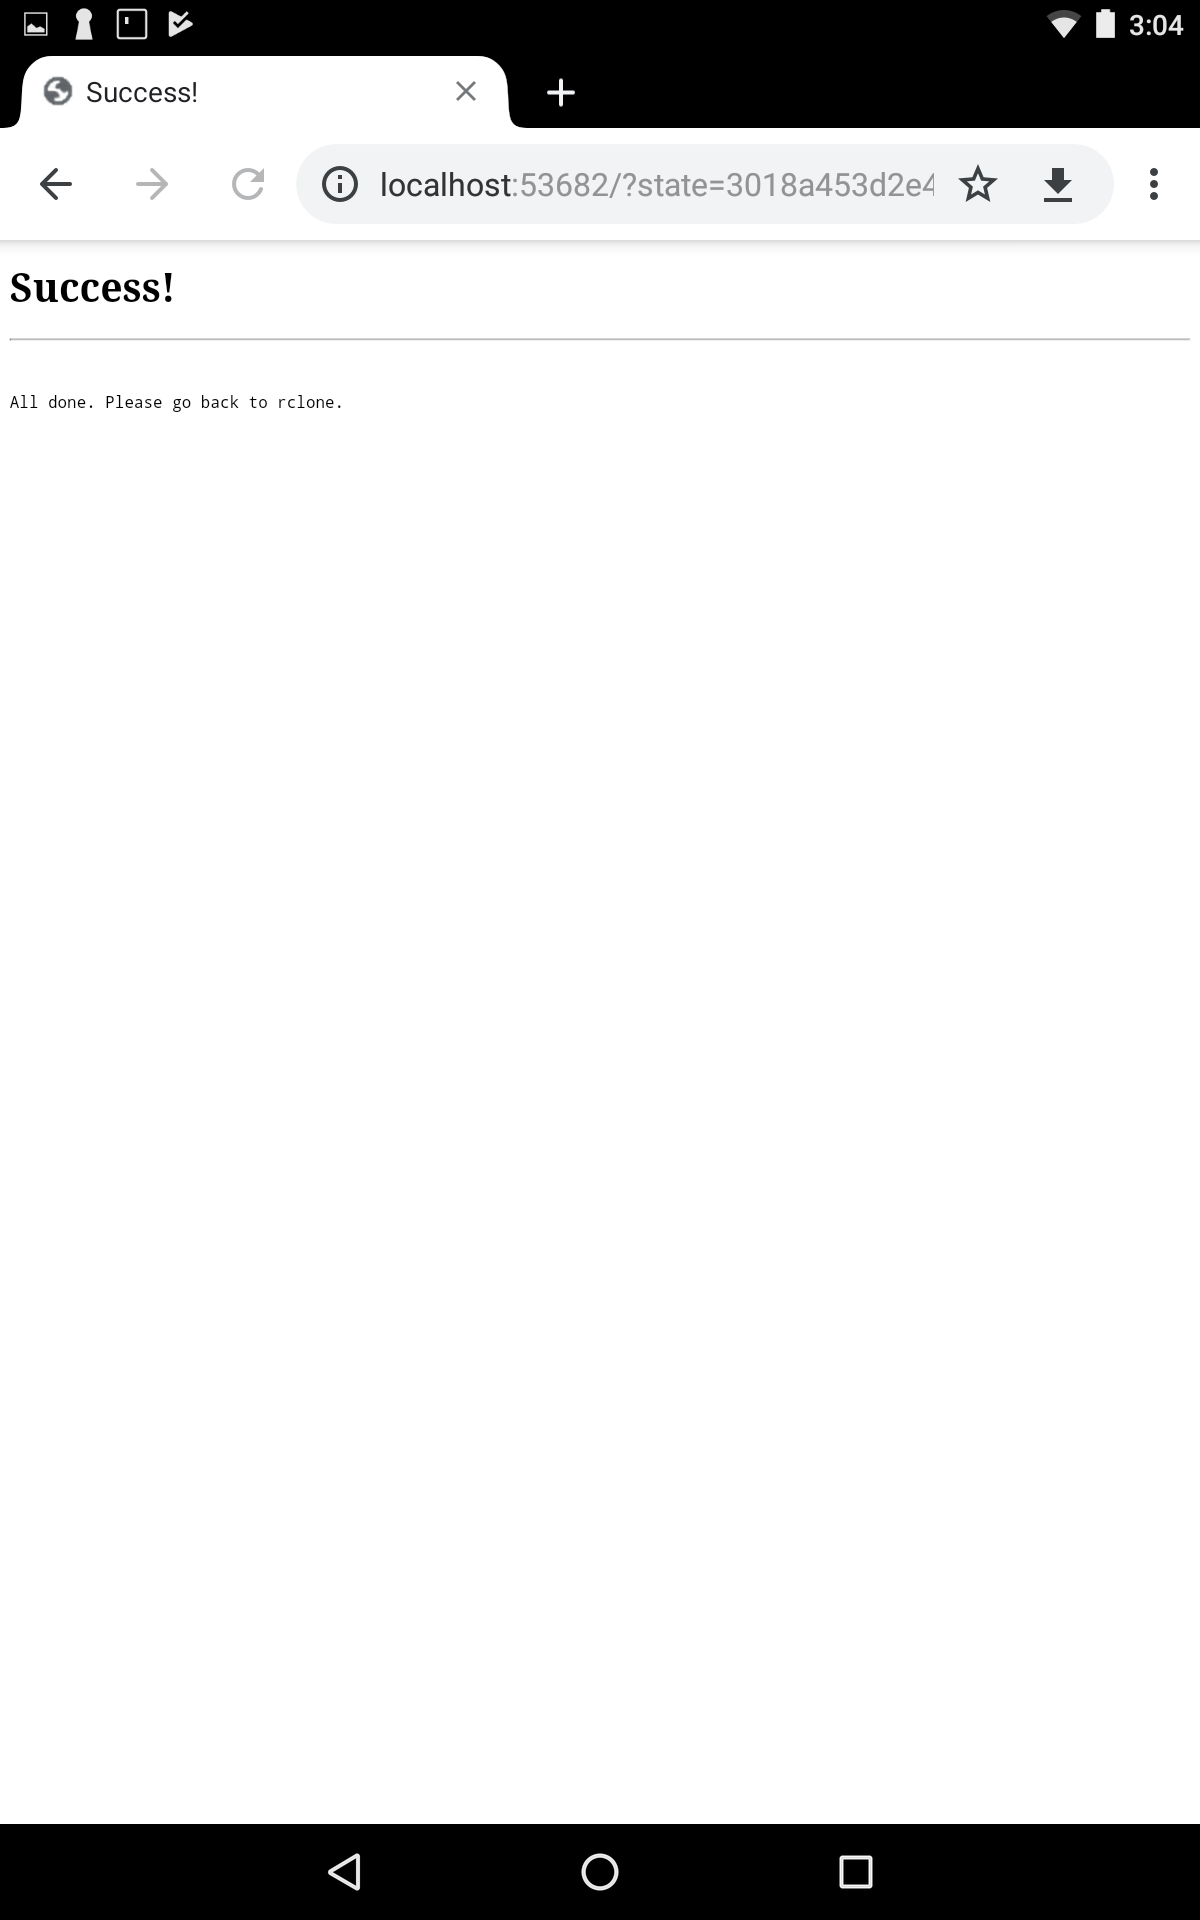
\includegraphics[scale=0.2]{images/dropbox3.png}
  \caption{RClone is successfully connected to Dropbox}
  \label{fig:dropbox3}
\end{figure}
\section{Microsoft OneDrive}
Next, I move on to Microsoft OneDrive to demonstrate that RClone has implemented mounting for directories and files stored in the OneDrive cloud storage provider. The following is the terminal output.\\
\begin{verbatim}
$ rclone config
Current remotes:

Name                 Type
====                 ====
dpremote             dropbox
remote               drive

e) Edit existing remote
n) New remote
d) Delete remote
r) Rename remote
c) Copy remote
s) Set configuration password
q) Quit config
e/n/d/r/c/s/q> n
name> onedremote
Type of storage to configure.
Enter a string value. Press Enter for the default ("").
Choose a number from below, or type in your own value
1 / A stackable unification remote, which can appear to merge the 
contents of several remotes
   \ "union"
2 / Alias for an existing remote
   \ "alias"
3 / Amazon Drive
   \ "amazon cloud drive"
4 / Amazon S3 Compliant Storage Provider (AWS, Alibaba, Ceph, 
Digital Ocean, Dreamhost, IBM COS, Minio, etc)
   \ "s3"
5 / Backblaze B2
   \ "b2"
6 / Box
   \ "box"
7 / Cache a remote
   \ "cache"
8 / Dropbox
   \ "dropbox"
9 / Encrypt/Decrypt a remote
   \ "crypt"
10 / FTP Connection
   \ "ftp"
11 / Google Cloud Storage (this is not Google Drive)
   \ "google cloud storage"
12 / Google Drive
   \ "drive"
13 / Hubic
   \ "hubic"
14 / JottaCloud
   \ "jottacloud"
15 / Koofr
   \ "koofr"
16 / Local Disk
   \ "local"
17 / Mega
   \ "mega"
18 / Microsoft Azure Blob Storage
   \ "azureblob"
19 / Microsoft OneDrive
   \ "onedrive"
20 / OpenDrive
   \ "opendrive"
21 / Openstack Swift (Rackspace Cloud Files, Memset Memstore, OVH)
   \ "swift"
22 / Pcloud
   \ "pcloud"
23 / QingCloud Object Storage
   \ "qingstor"
24 / SSH/SFTP Connection
   \ "sftp"
25 / Webdav
   \ "webdav"
26 / Yandex Disk
   \ "yandex"
27 / http Connection
   \ "http"
Storage> onedrive
** See help for onedrive backend at: https://rclone.org/onedrive/ **

Microsoft App Client Id
Leave blank normally.
Enter a string value. Press Enter for the default ("").
client_id>
Microsoft App Client Secret
Leave blank normally.
Enter a string value. Press Enter for the default ("").
client_secret>
Edit advanced config? (y/n)
y) Yes
n) No
y/n> y
Chunk size to upload files with - must be multiple of 320k.

Above this size files will be chunked - must be multiple of 320k. Note
that the chunks will be buffered into memory.
Enter a size with suffix k,M,G,T. Press Enter for the default ("10M").
chunk_size>
The ID of the drive to use
Enter a string value. Press Enter for the default ("").
drive_id>
The type of the drive ( personal | business | documentLibrary )
Enter a string value. Press Enter for the default ("").
drive_type>
Set to make OneNote files show up in directory listings.

By default rclone will hide OneNote files in directory listings because
operations like "Open" and "Update" won't work on them.  But this
behaviour may also prevent you from deleting them.  If you want to
delete OneNote files or otherwise want them to show up in directory
listing, set this option.
Enter a boolean value (true or false). Press Enter for the default 
("false").
expose_onenote_files>
Remote config
Use auto config?
* Say Y if not sure
* Say N if you are working on a remote or headless machine
y) Yes
n) No
y/n> y
If your browser doesn't open automatically go to the following link: 
http://127.0.0.1:53682/auth
Log in and authorize rclone for access
Waiting for code...
Got code
Choose a number from below, or type in an existing value
1 / OneDrive Personal or Business
   \ "onedrive"
2 / Root Sharepoint site
   \ "sharepoint"
3 / Type in driveID
   \ "driveid"
4 / Type in SiteID
   \ "siteid"
5 / Search a Sharepoint site
   \ "search"
Your choice> onedrive
Found 1 drives, please select the one you want to use:
0: OneDrive (business) id=b!AmMSbuU0XECVJSfFj3kIDHna4T8RxlZDhahlLNJ3
l55RInJ4tOvLToGs8g0fShDA
Chose drive to use:> 0
Found drive 'root' of type 'business', URL: https://raidermailwright-
my.sharepoint.com/personal/
alkhafaji_2_wright_edu/Documents
Is that okay?
y) Yes
n) No
y/n> y
--------------------
[onedremote]
type = onedrive
token = {"access_token":"xxxxxxxxxxxxxxxxxxxxxx-_xx-xxxxxxxxxxxxxxxxxx
-49n9Z6wpz-MQlU7XztJKgeWzo_-xxxxxxxxxxx","token_type":"Bearer",
"refresh_token":"OAQABAAAAAAAxxxxx-xxxxxx-SyE93jJKbUL7nz-xxxxxx-
yKw4be8aK4g-xxxxxxxxxxxxxxxxxx","expiry":
"2019-08-05T20:11:01.044813516Z"}
drive_id = b!AmMSbuU0XECVJSfFj3kIDHna4T8RxlZDhahlLNJ3l55RInJ4tOvL
ToGs8g0fShDA
drive_type = business
--------------------
y) Yes this is OK
e) Edit this remote
d) Delete this remote
y/e/d> y
\end{verbatim}
Refer to Figure \ref{fig:onedrive1}, Figure \ref{fig:onedrive2}, and Figure \ref{fig:onedrive3} for visualization of what occurs when the browser appears when user runs the commands above.
\begin{figure}[htb]
  \centering
  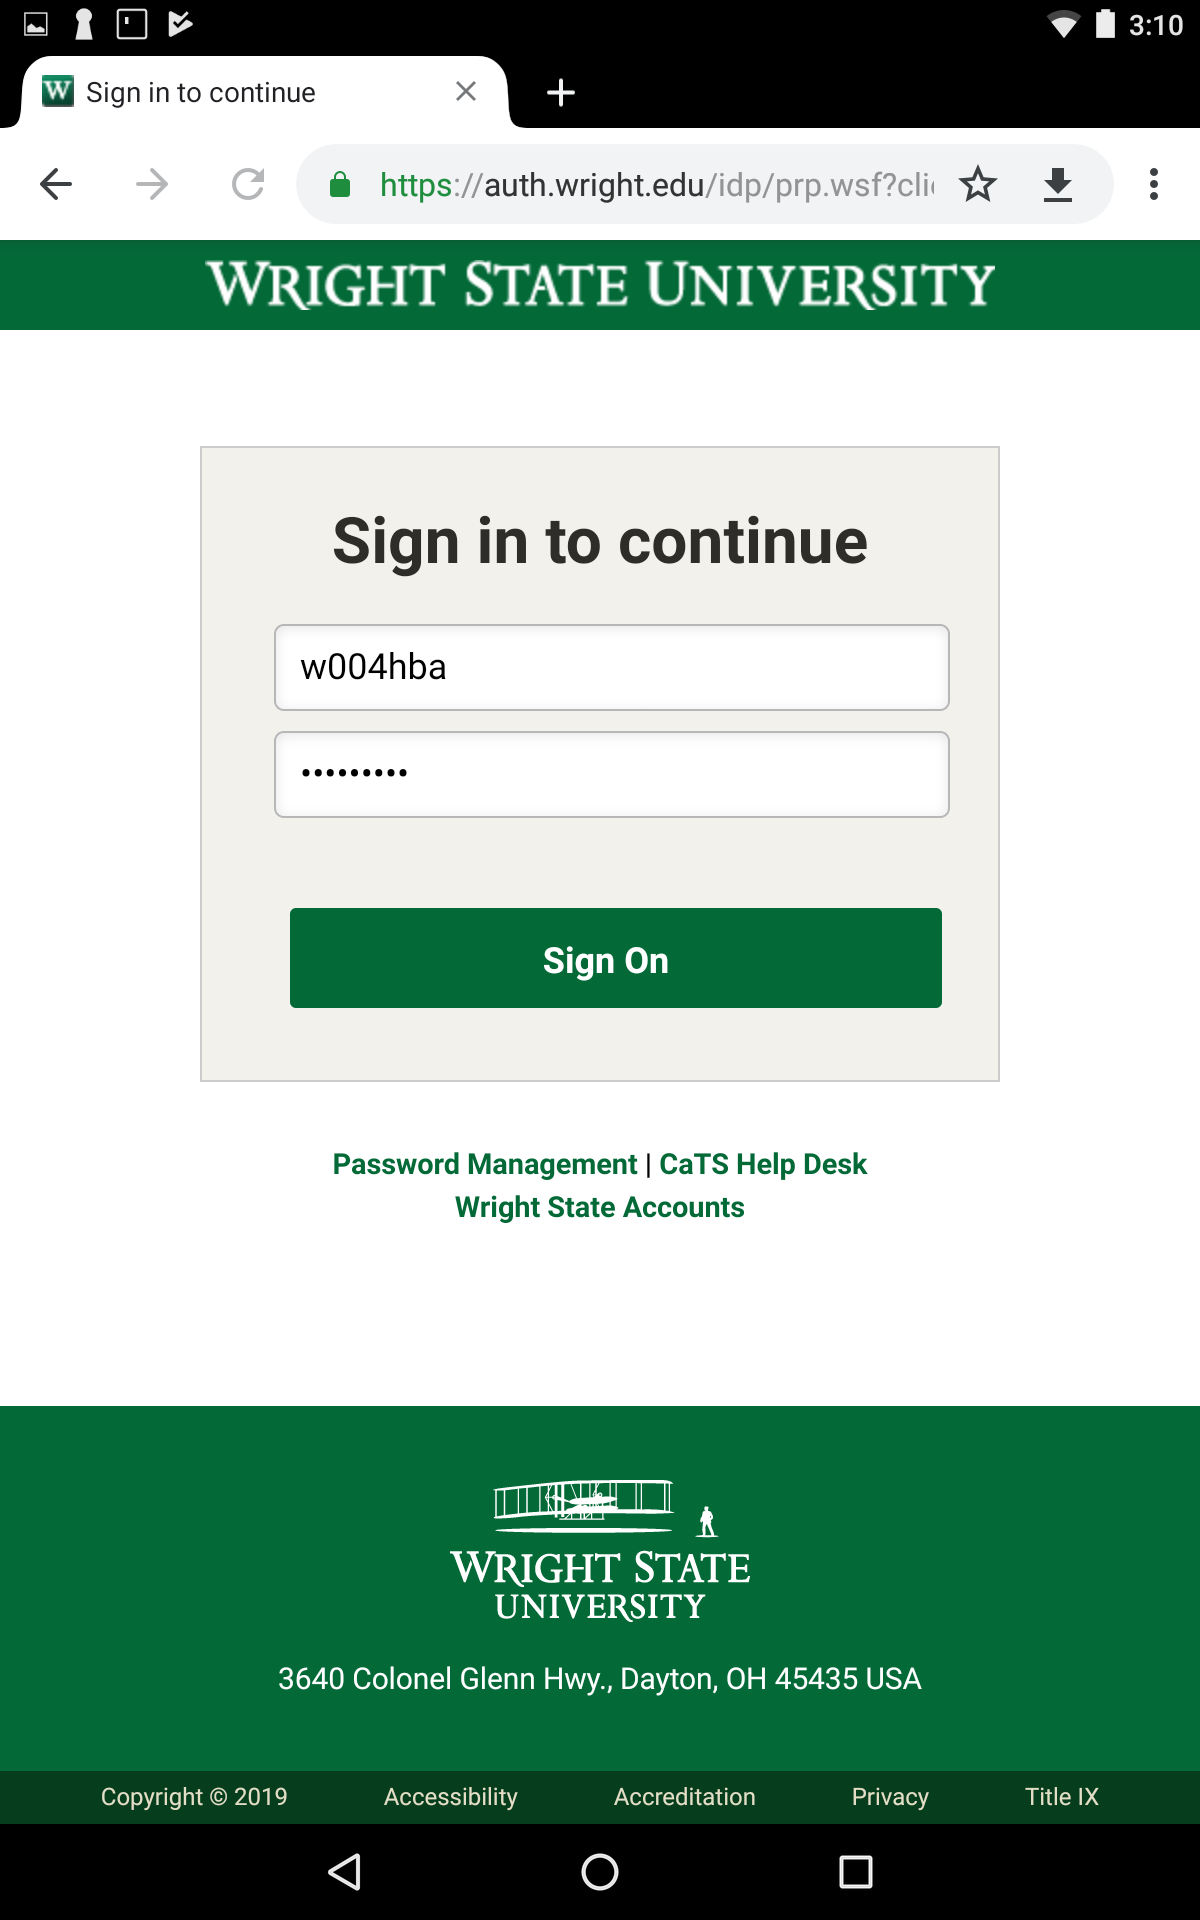
\includegraphics[scale=0.2]{images/onedrive1.png}
  \caption{Browser appears prompting for OneDrive credentials}
  \label{fig:onedrive1}
\end{figure}
\begin{figure}[htb]
  \centering
  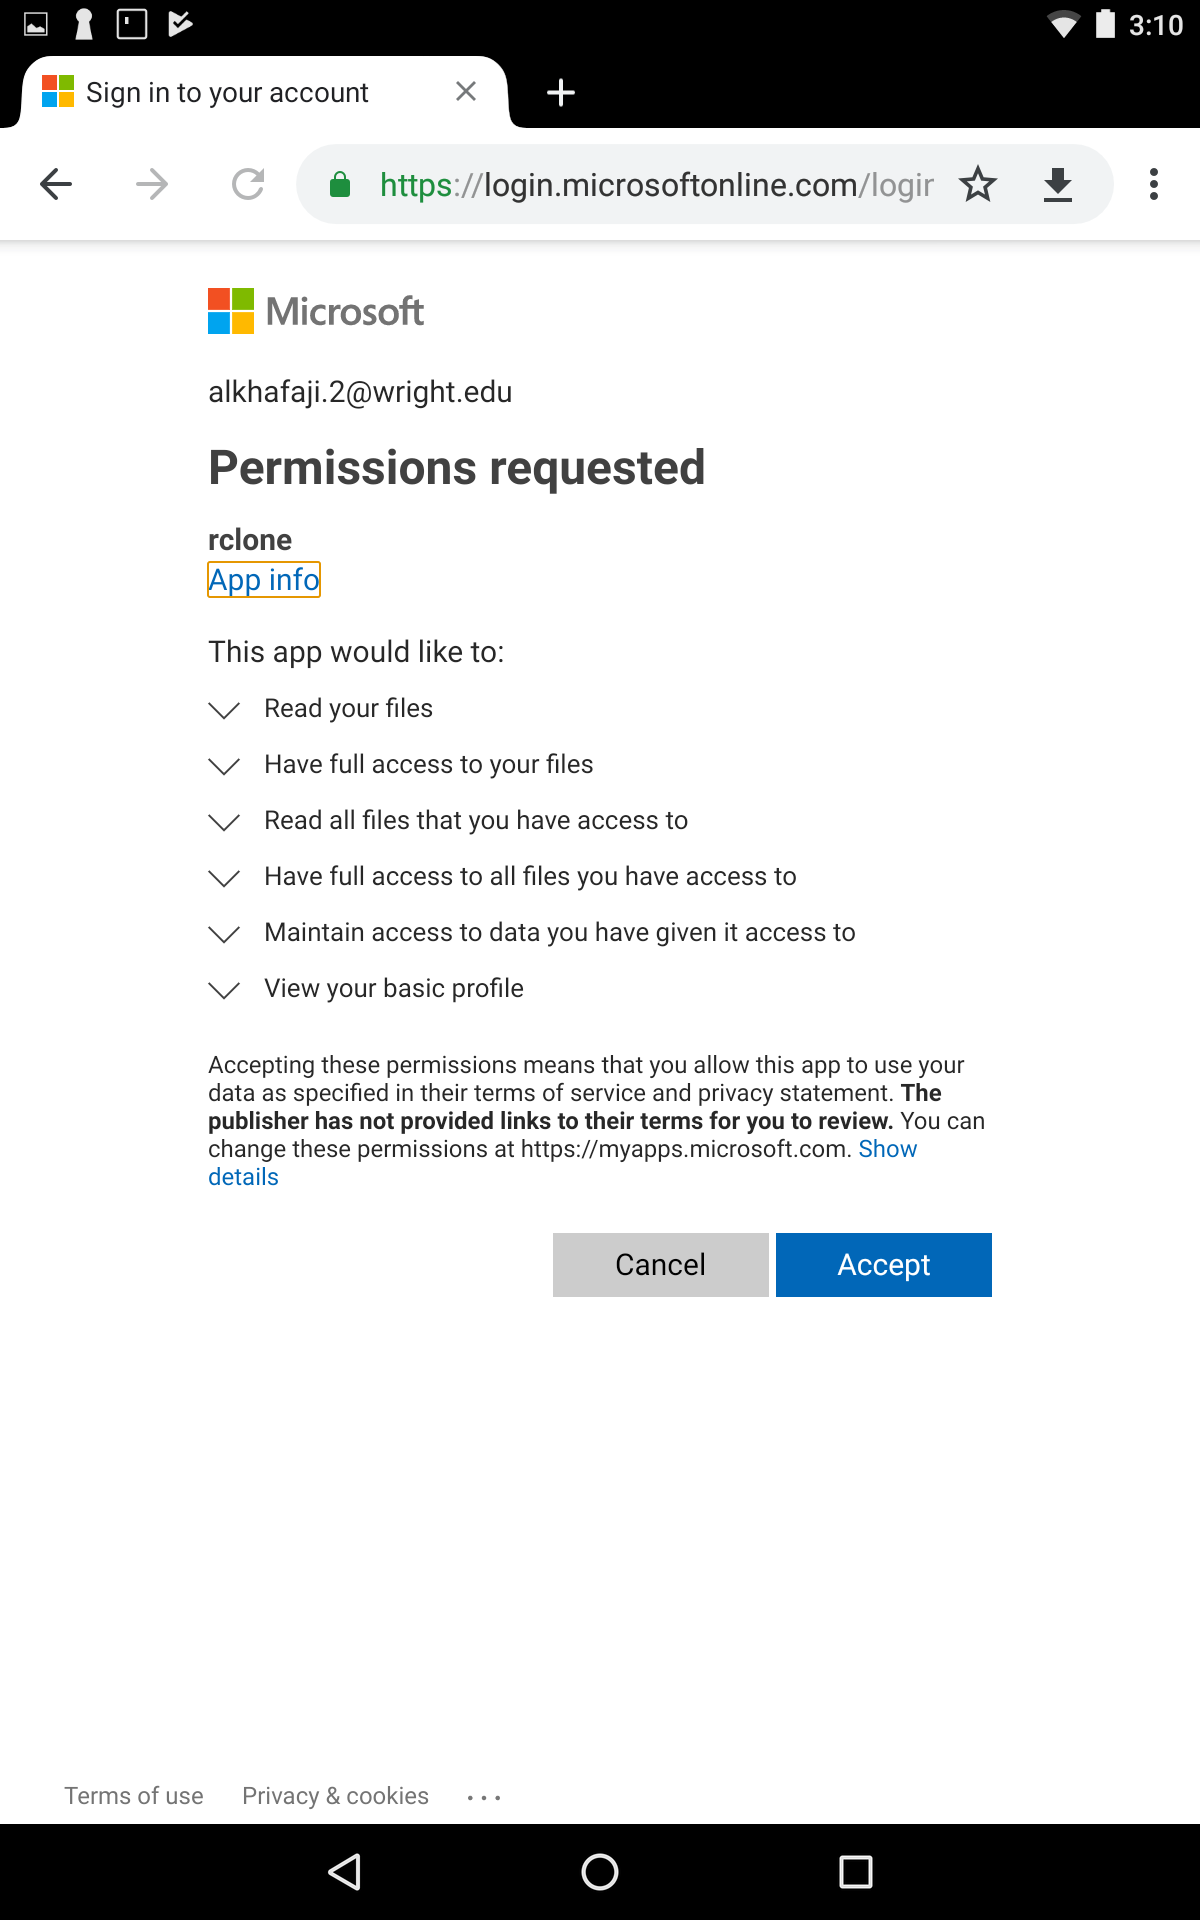
\includegraphics[scale=0.2]{images/onedrive2.png}
  \caption{RClone requests permission to access OneDrive content}
  \label{fig:onedrive2}
\end{figure}
\begin{figure}[htb]
  \centering
  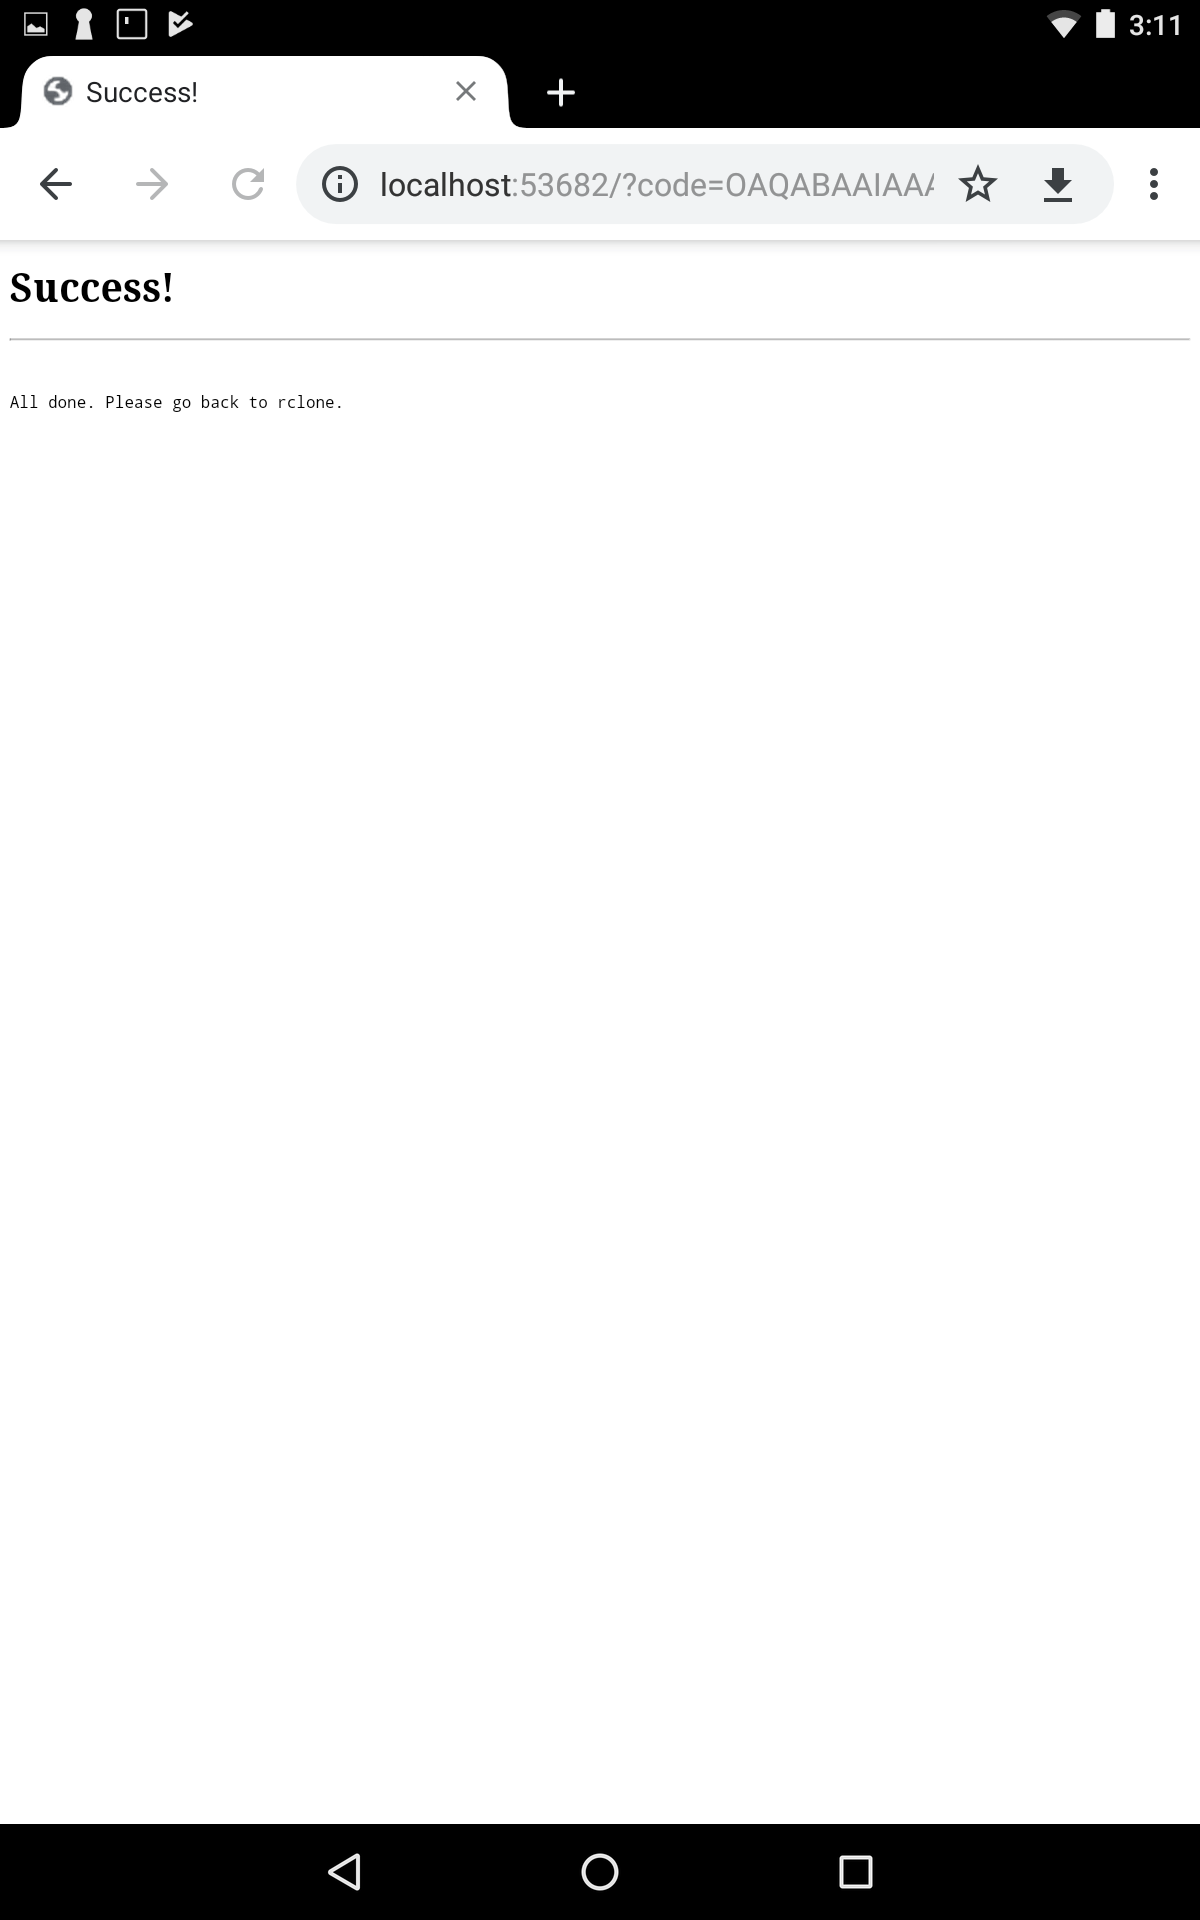
\includegraphics[scale=0.2]{images/onedrive3.png}
  \caption{RClone is successfully connected to OneDrive}
  \label{fig:onedrive3}
\end{figure}
\section{pCloud}
Next, I move on to pCloud to demonstrate that RClone has implemented mounting for directories and files stored in the pCloud storage provider. The following is the terminal output.\\
\begin{verbatim}
$ rclone config
Current remotes:

Name                 Type
====                 ====
dpremote             dropbox
onedremote           onedrive
remote               drive

e) Edit existing remote
n) New remote
d) Delete remote
r) Rename remote
c) Copy remote
s) Set configuration password
q) Quit config
e/n/d/r/c/s/q> n
name> pcloudremote
Type of storage to configure.
Enter a string value. Press Enter for the default ("").
Choose a number from below, or type in your own value
1 / A stackable unification remote, which can appear to merge the 
contents of several remotes
   \ "union"
2 / Alias for an existing remote
   \ "alias"
3 / Amazon Drive
   \ "amazon cloud drive"
4 / Amazon S3 Compliant Storage Provider (AWS, Alibaba, Ceph, 
Digital Ocean, Dreamhost, IBM COS, Minio, etc)
   \ "s3"
5 / Backblaze B2
   \ "b2"
6 / Box
   \ "box"
7 / Cache a remote
   \ "cache"
8 / Dropbox
   \ "dropbox"
9 / Encrypt/Decrypt a remote
   \ "crypt"
10 / FTP Connection
   \ "ftp"
11 / Google Cloud Storage (this is not Google Drive)
   \ "google cloud storage"
12 / Google Drive
   \ "drive"
13 / Hubic
   \ "hubic"
14 / JottaCloud
   \ "jottacloud"
15 / Koofr
   \ "koofr"
16 / Local Disk
   \ "local"
17 / Mega
   \ "mega"
18 / Microsoft Azure Blob Storage
   \ "azureblob"
19 / Microsoft OneDrive
   \ "onedrive"
20 / OpenDrive
   \ "opendrive"
21 / Openstack Swift (Rackspace Cloud Files, Memset Memstore, OVH)
   \ "swift"
22 / Pcloud
   \ "pcloud"
23 / QingCloud Object Storage
   \ "qingstor"
24 / SSH/SFTP Connection
   \ "sftp"
25 / Webdav
   \ "webdav"
26 / Yandex Disk
   \ "yandex"
27 / http Connection
   \ "http"
Storage> pcloud
** See help for pcloud backend at: https://rclone.org/pcloud/ **

Pcloud App Client Id
Leave blank normally.
Enter a string value. Press Enter for the default ("").
client_id>
Pcloud App Client Secret
Leave blank normally.
Enter a string value. Press Enter for the default ("").
client_secret>
Remote config
Use auto config?
* Say Y if not sure
* Say N if you are working on a remote or headless machine
y) Yes
n) No
y/n> y
If your browser doesn't open automatically go to the following link: 
http://127.0.0.1:53682/auth
Log in and authorize rclone for access
Waiting for code...
Got code
--------------------
[pcloudremote]
type = pcloud
token = {"access_token":"Jc0rZDnONSzyJXpmZOIo7N7Zgm5qYeGg5qHLaLt
TCoV9pjdXsQHy","token_type":"bearer","expiry":
"0001-01-01T00:00:00Z"}
--------------------
y) Yes this is OK
e) Edit this remote
d) Delete this remote
y/e/d> y
\end{verbatim}
Refer to Figure \ref{fig:pcloud1}, Figure \ref{fig:pcloud2}, and Figure \ref{fig:pcloud3} for visualization of what occurs when the browser appears when user runs the commands above.
\begin{figure}[htb]
  \centering
  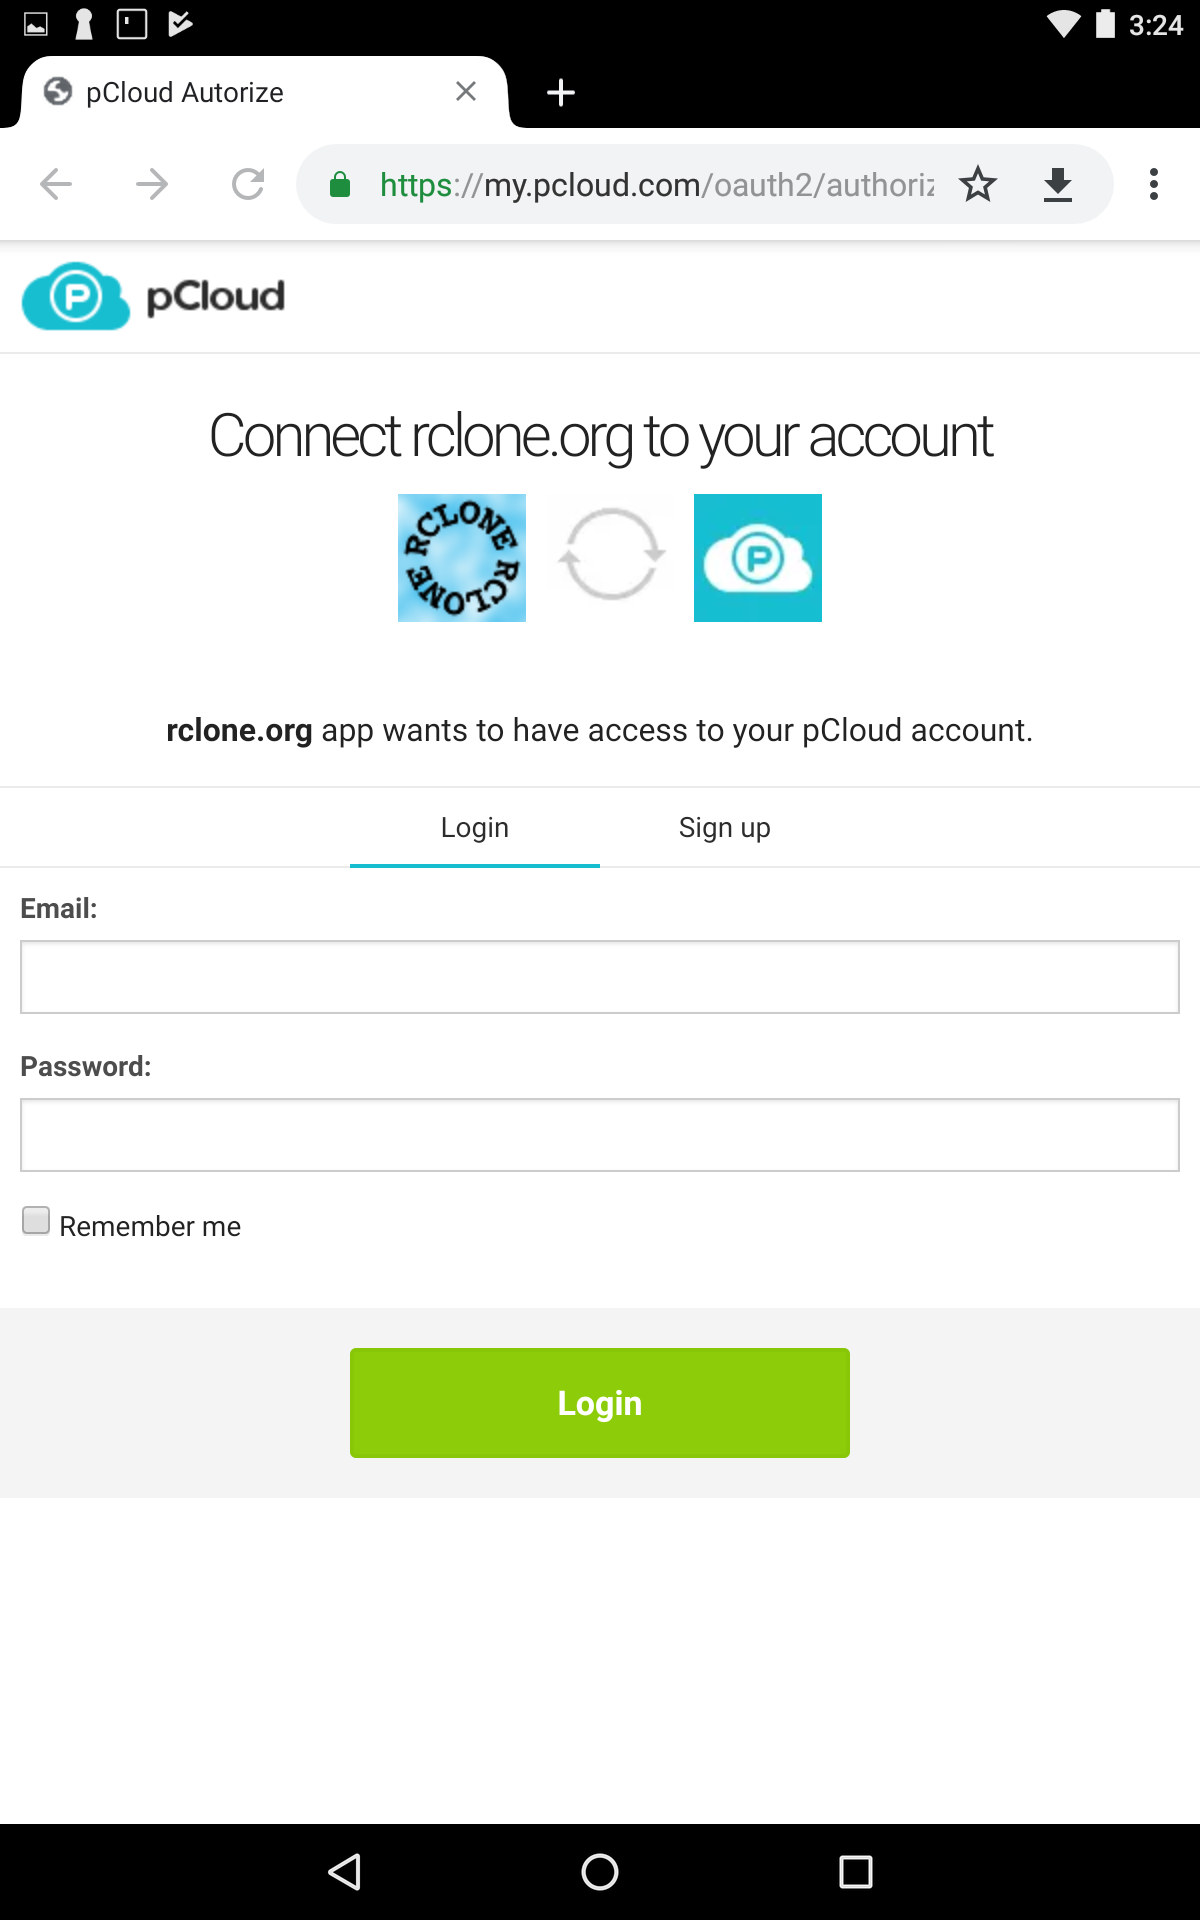
\includegraphics[scale=0.2]{images/pcloud1.png}
  \caption{Browser appears prompting for pCloud credentials}
  \label{fig:pcloud1}
\end{figure}
\begin{figure}[htb]
  \centering
  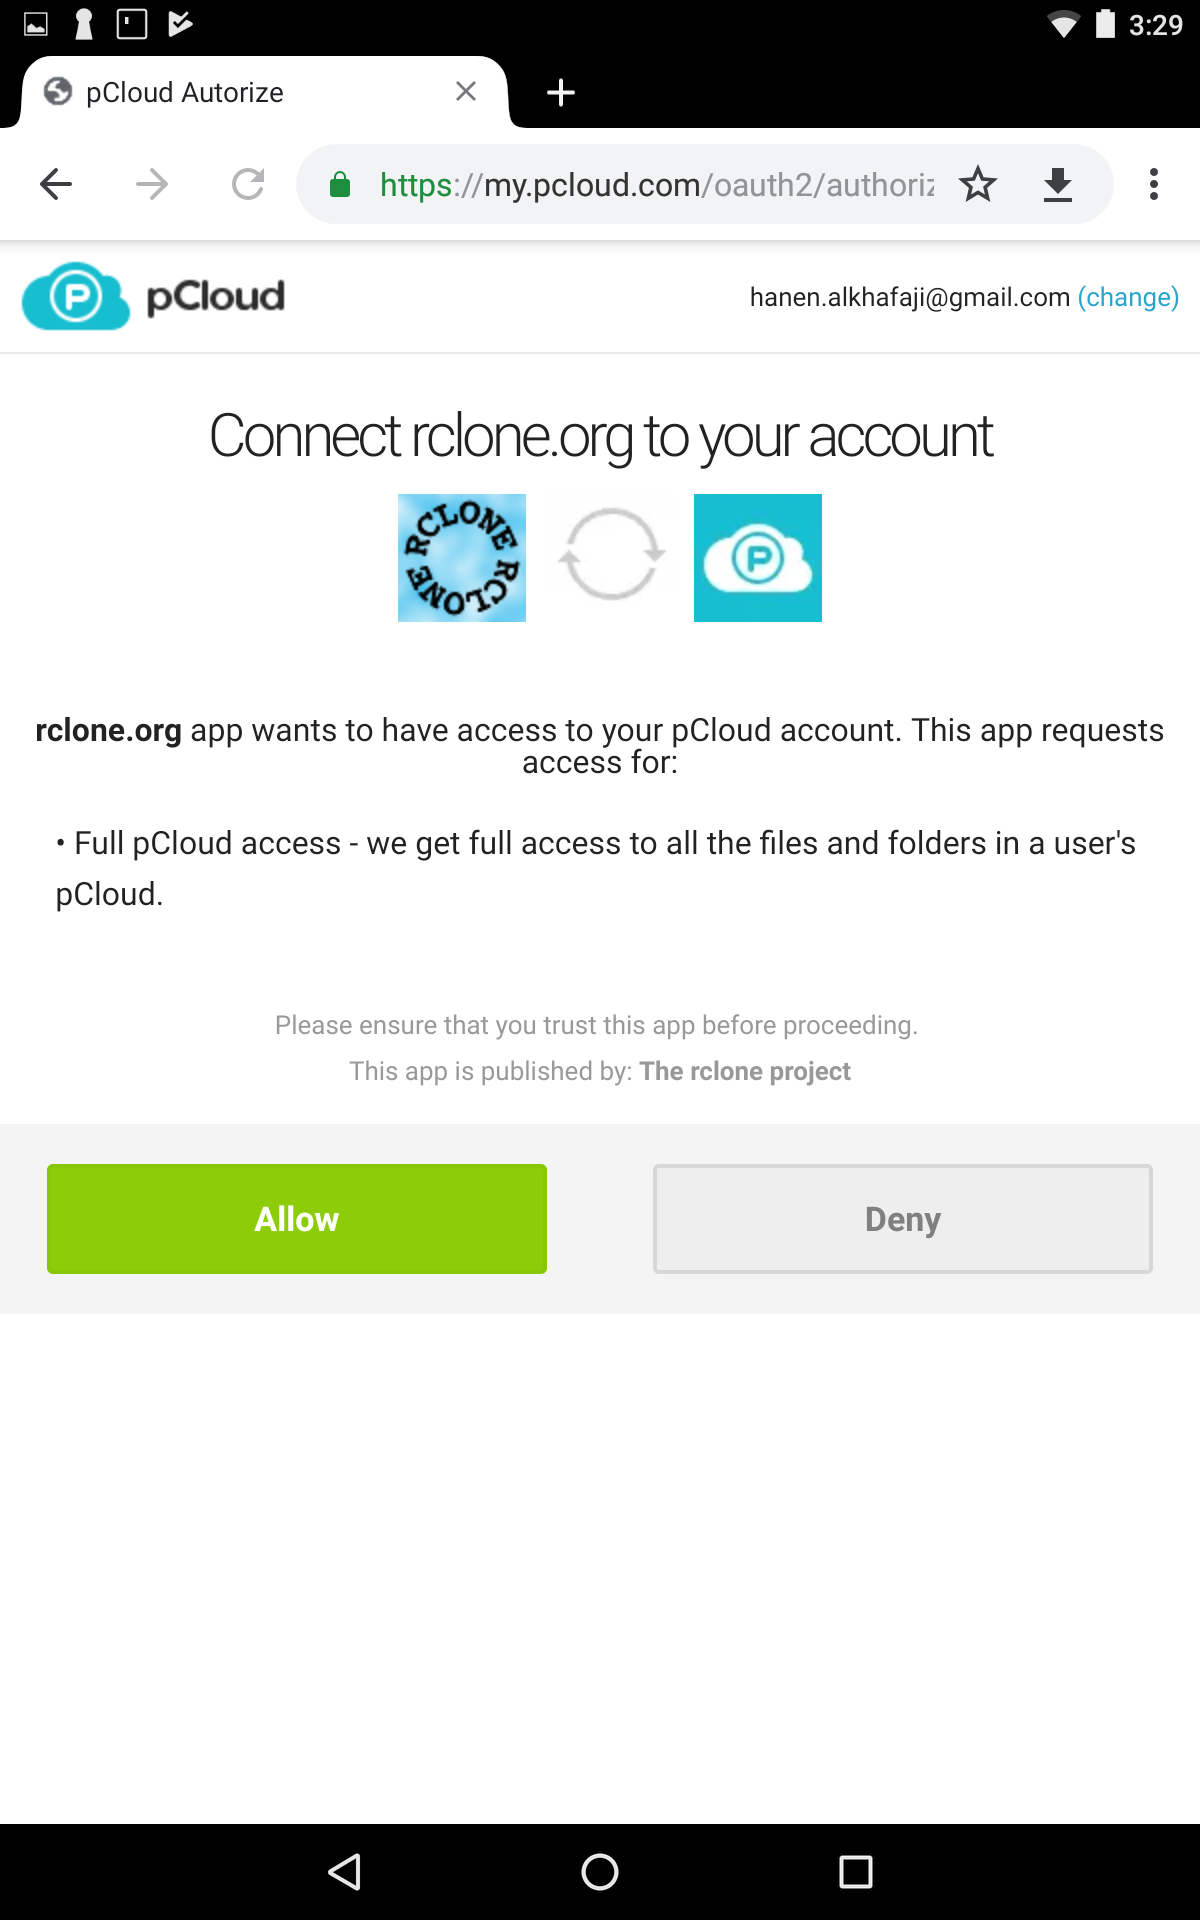
\includegraphics[scale=0.2]{images/pcloud2.png}
  \caption{RClone requests permission to access pCloud content}
  \label{fig:pcloud2}
\end{figure}
\begin{figure}[htb]
  \centering
  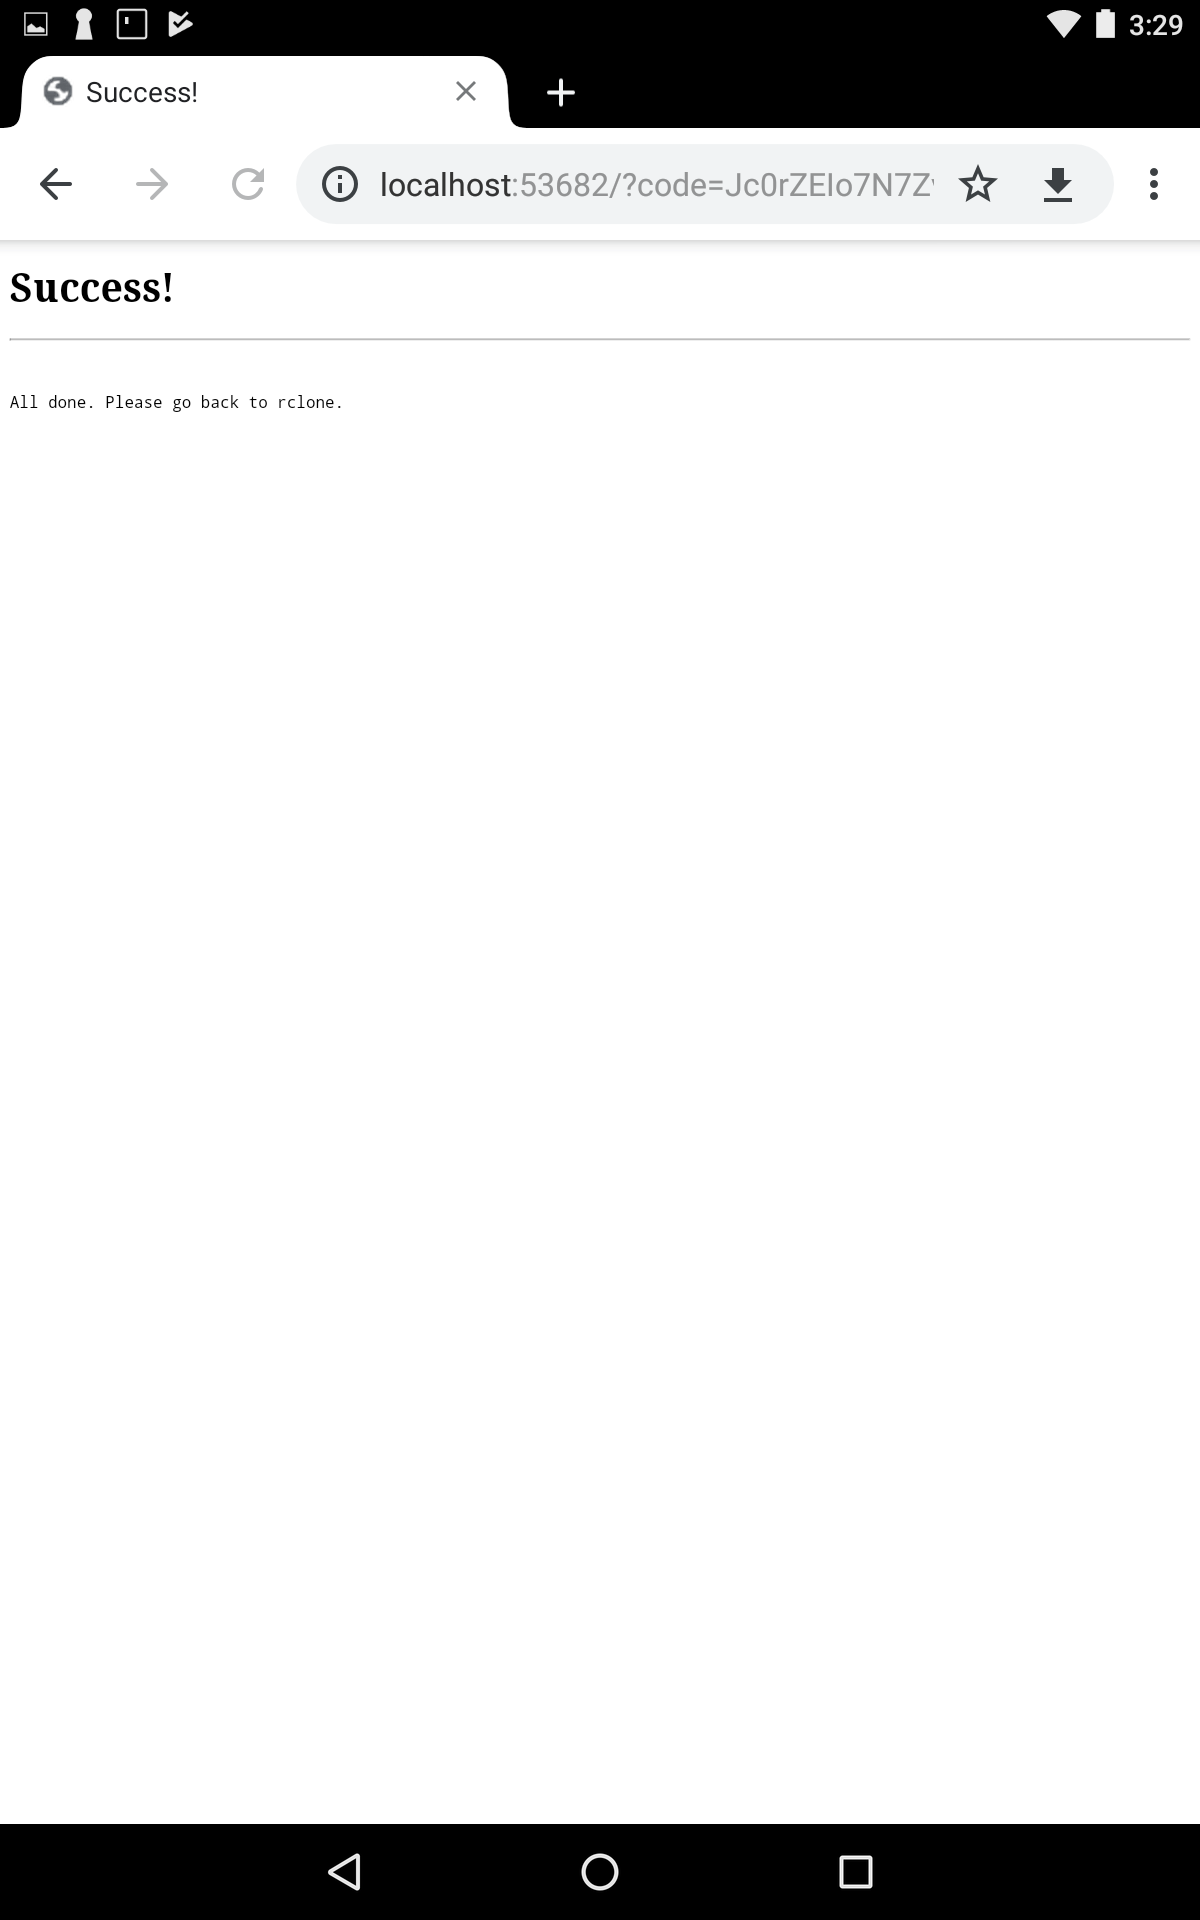
\includegraphics[scale=0.2]{images/pcloud3.png}
  \caption{RClone is successfully connected to pCloud}
  \label{fig:pcloud3}
\end{figure}